
\section{AMR Spatial Discretization} \label{sect:AMRnotation}

The underlying discretization of space is given as points 
$(i_0, ... , i_{\Dim - 1}) = \ibold \in \mathbb{Z}^\Dim$. 
The problem domain is discretized using a grid 
$\Gamma \subset {\mathbb{Z}}^\Dim$
that is a bounded subset of the lattice.
$\Gamma$ is used to represent a cell-centered
discretization of the continuous spatial domain into a collection of
control volumes:  ${\ibold} \in \Gamma$ represents a
region of space $[\xbold_0 + (\ibold - \half
\ubold)h, \xbold_0 + (\ibold + \half
\ubold)h]$, where $\xbold_0 \in \mathbb{R}^\Dim$ is some fixed origin of
coordinates, $h$ is the mesh spacing, and $\ubold \in
{\mathbb{Z}}^\Dim$ is the vector whose components are all equal to one.
We can also define various face-centered and node-centered
discretizations of space based on those control volumes.  For example,
we denote by $\Gamma^{\vbold}$ the set of points in physical
space of the form $\xbold_0 + (\ibold \pm \half \vbold)
h, \ibold \in \Gamma$.  Here $\vbold$ can be any
vector whose entries are equal to either zero or one.

We will find it useful to define a number of operators on points and
subsets of $\mathbb{Z}^\Dim$. 
We denote by $|\ibold| = \underset{d = 0 \dots \Dim - 1}{max}(|i_d|)$, 
$\Gamma + \ibold$ as the translation of a set by a point in
${\mathbb{Z}}^\Dim$, and $\mathcal{G}(\Gamma,r)$ to the set of all points
within a $|\cdot|$-distance $r$ of $\Gamma$
\beqa
\mathcal{G}(\Gamma,r) = \underset{|\ibold| \leq r}{\cup} \Gamma +
\ibold
\eeqa
We define a coarsening operator by
${\mathcal{C}}_r : {\mathbb{Z}}^\Dim \rightarrow {\mathbb{Z}}^\Dim$,
\beqa
{\mathcal{C}}_r(\ibold) = (\lfloor \frac{i_0}{r} \rfloor,..., \lfloor
\frac{i_{d-1}}{r} \rfloor)
\eeqa
where r is a positive integer.
The coarsening operator acting on subsets of $\mathbb{Z}^\Dim$ can be
extended in a natural way to the other grid centerings:  
${\mathcal{C}}_r(\Gamma^{\vbold}) \equiv ({\mathcal{C}}_r(\Gamma))^{\vbold}$.

We extend this discretization of space to represent a nested hierarchy of grids
that discretize the same continuous spatial domain.
We assume that our problem domain can be discretized by a nested
hierarchy of grids $\Gamma^0 ... \Gamma^{lmax}$, with $\Gamma^{l+1} = 
{\mathcal{C}}^{-1}_{n^l_{ref}}(\Gamma^l)$, and
$\xbold^l_0 - \half \ubold h^l$ independent of $l$.  The integer $n^l_{ref}$ is
the refinement ratio between level $l$ and $l+1$.  We also assume that
the mesh spacings $h^l$ associated with $\Gamma^l$ satisfy
$\frac{h^l}{h^{l+1}} = n^l_{ref}$.  These conditions imply that the
underlying continuous spatial domains defined by the control volumes 
are all identical.

Adaptive mesh refinement calculations are
performed on a hierarchy of meshes $\Omega^\ell \subset \Gamma^\ell$, with
$\Omega^\ell \supset {\mathcal{C}}_{n^\ell_{ref}}(\Omega^{\ell+1})$.
Typically, $\Omega^l$ is decomposed into a disjoint union of
rectangles in order to perform calculations efficiently.  We denote
such a decomposition by ${\mathcal{R}}(\Omega^l) = \{ \Omega^l_k
\}^{N^l_{grids}}_{k=1}$, where the $\Omega^l_k$'s are rectangles and
$\Omega^l_k \cap \Omega^l_{k'} = \emptyset \mbox{ if } k \neq k'$.  We say
that ${\mathcal{R}}(\Omega^l)$ is $p$-blocked, $p>1$, if
$\Omega^l_k = {\mathcal{C}}^{-1}_p({\mathcal{C}}_p(\Omega^l_k))$ for
all $k$.  We will assume throughout that $\Omega^l$ admits a
decomposition ${\mathcal{R}}(\Omega^l)$ that is
$n^{l-1}_{ref}$-blocked for all $l>0$.  In particular, the control volume
corresponding to a cell in $\Omega^{l-1}$ is either completely
contained in the control volumes defined by $\Omega^l$ or its
intersection has zero volume. We will also assume that there is at least
one level $l$ cell separating level $l+1$ cells from level $l-1$ cells:
$\mathcal{G}(\mathcal{C}_{n^l_{nref}}(\Omega^{l+1}),1) \cap \Gamma^l \subseteq
\Omega^l$. We will refer to grid hierarchies that meet 
these two conditions as being
{\it properly nested}. We emphasize that this form of proper nesting is
a minimum requirement for the AMR algorithms discussed in this document.
For some applications, it may be necessary to impose more stringent
conditions on the grid hierarchy.

A discretized dependent variable in AMR is a {\it level array} 
\beqa
\varphi^l : \Omega^l \rightarrow {\mathbb{R}}^m
\eeqa
We denote by $\varphi_\ibold
\in {\mathbb{R}}^m$ the value of $\varphi$ at cell $\ibold \in
\Omega^l$.  We can also define level arrays on other grid centerings,
i.e., $\psi:\Omega^{l,\vbold} \rightarrow {\mathbb{R}}^m$. In that case,
we denote the indexing operation by $\psi_{\ibold + \half \vbold} \in
\mathbb{R}^m$. In particular, we can define vector fields
at a level
\beqa
\vec{F}^l = (F_0^l, ..., F^l_{\Dim-1}) \hbox{ , } F^l_d : \Omega^{l, \ebold^d}
\rightarrow {\mathbb{R}}^m
\eeqa

\begin{figure}[htp]
\centerline{
%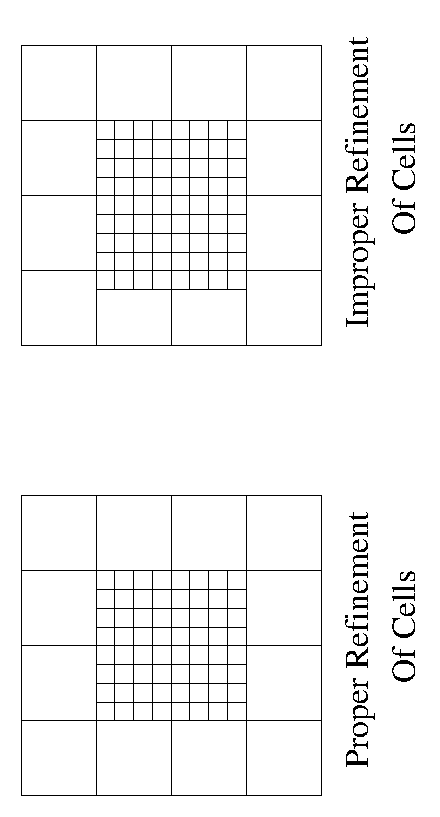
\epsfig{file=figs/propernest.req.1.eps,angle=270,width=3.0in}
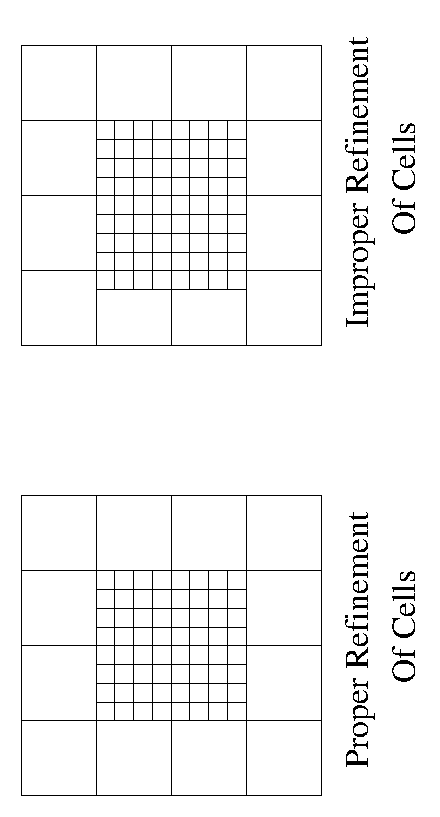
\includegraphics[type=eps,ext=.eps,read=.eps]{figs/propernest.req.1}
%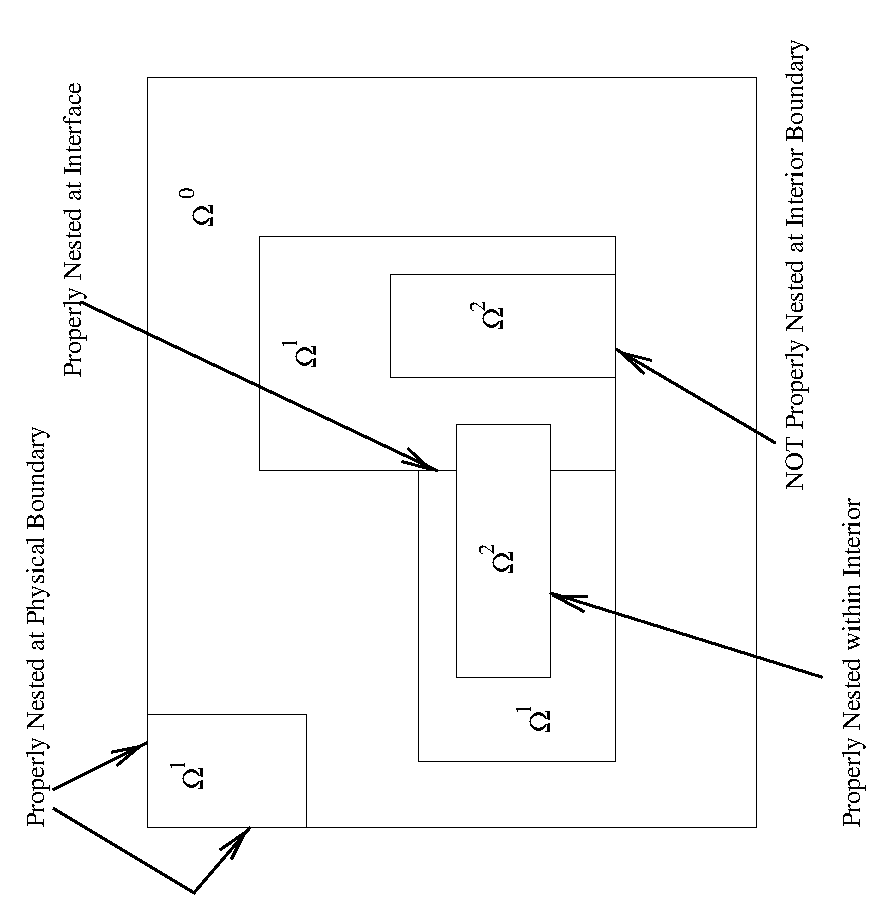
\epsfig{file=figs/propernest.req.2.eps,angle=270,width=3.0in}}
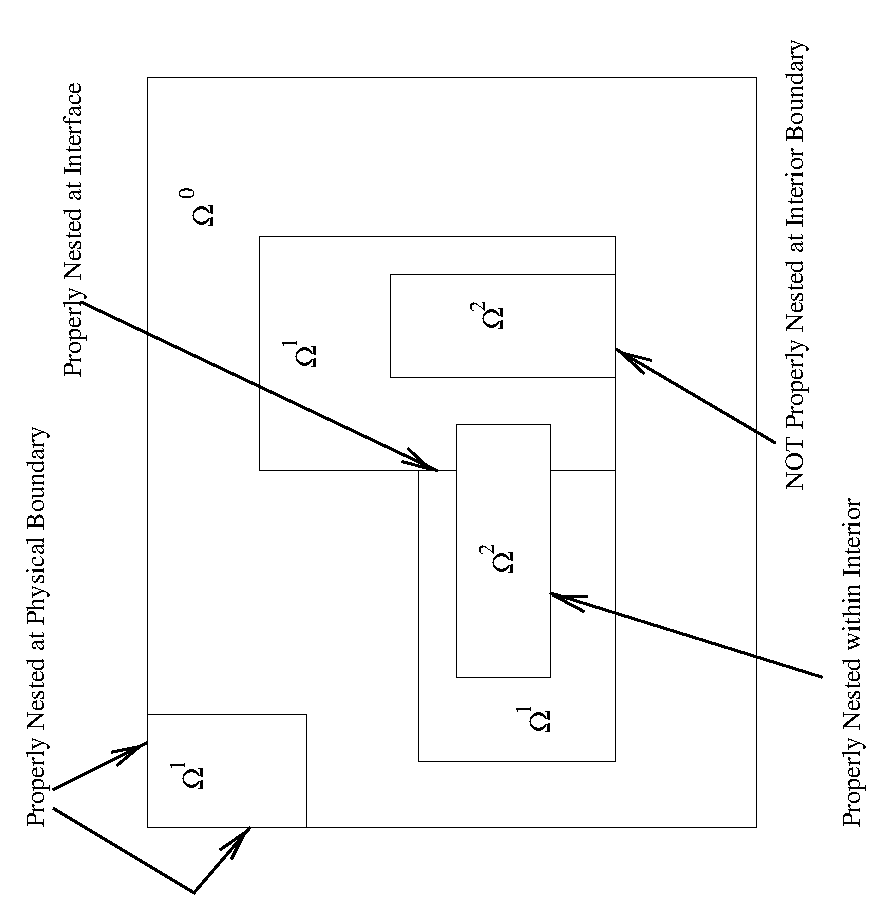
\includegraphics[type=eps,ext=.eps,read=.eps]{figs/propernest.req.2}
}
\caption{Examples illustrating proper nesting requirements for 
locally refined grids.}
\label{fig:basicAMRPic}
\end{figure}

We will be interested in operations on pairs of refined grids that
are not necessarily contained in an AMR mesh hierarchy (e.g., during
regridding). In those cases, we
will denote by $\Gamma^f$, $\Gamma^c$ the fine and coarse problem
domains, $n_{ref}$ the refinement ratio between the two levels, 
$\Omega^f$, $\Omega^c$ the refined regions in the two domains, and 
$\varphi^f$, $\varphi^c$, etc., level arrays defined on $\Omega^f$,
$\Omega^c$. We will always assume that the two levels are properly
nested.

In the remainder of this section, we will describe {\it BoxTools},
a set of abstractions for defining points and regions in a
multidimensional integer lattice index space, and representing
aggregate data in such regions. 
The classes defined in the remainder of this chapter correspond to the
mathematical objects described above in the following fashion.
\begin{trivlist}
\item $\bullet$
Points in the rectangular lattice $\ibold \in \mathbb{Z}^\Dim$ 
$\Leftrightarrow$ the class {\tt IntVect}.
\item $\bullet$
Rectangular subsets $\Gamma \subset \mathbb{Z}^\Dim$ $\Leftrightarrow$
the class {\tt Box}.
\item $\bullet$
Arbitrary subsets $\mathcal{I} \subset \mathbb{Z}^\Dim$ $\Leftrightarrow$
the class {\tt IntVectSet}.
\item $\bullet$
Rectangular arrays $\varphi : \Gamma \rightarrow \mathbb{R}^m$
$\Leftrightarrow$ the class {\tt FArrayBox}.
\item $\bullet$
Unions of rectangles at a fixed level of refinement
$\Omega, \mathcal{R}(\Omega)$, and their distribution onto processors
$\Leftrightarrow$ the class
{\tt DisjointBoxLayout}.
\item $\bullet$
Level arrays $\varphi : \Omega \rightarrow \mathbb{R}^m$ $\Leftrightarrow$
the class {\tt LevelData<FArrayBox>}.
\end{trivlist}
